%%% Local Variables: 
%%% mode: latex
%%% TeX-master: "../main"
%%% End: 

\chapter{外文文献翻译}

标题:一种多阶段生产的控制方法——拉式生产的设计和分析

原标题:Design and analysis of Pull System, a method of multi-stage production control

作者:OSAMU KIMURA,HIROSUKE TERADA

摘要:我们把多阶段生产过程的控制系统分为两种,分别称它们为推式系统和拉式系统。前者是一种传统的方法——每个阶段库存的零部件是根据它到最终阶段的总流程时间来预测的。生产和库存控制是基于这些预测值的。后者是本文提出的一种方法——每个阶段保持一定总量的库存,其补给是根据后续生产过程的消耗速率而定的。我们先制定拉式系统的定义,然后从批量大小、提前期等系统参数出发,给出整个生产过程中的生产、库存波动的仿真模型。

\section{简介}

\subsection{传统生产订单系统及它面临的问题}

一般来说,由于制造需要的时间比允许的供货延迟时间长,多阶段制造过程需要预先生产一些产品。我们能把这些过程的生产控制系统归为以下两类。

\begin{enumerate}
\item
推式系统:这类系统考虑每个阶段到最终阶段的流程时间,预测每阶段库存零部件或在制材料的需求。基于这些预测,它们通过调整最终成品和零部件的库存来控制整个多阶段生产。我们把这一类称为推动型生产订单系统,或者简称推式系统。
\item
拉式系统:每个阶段保有一定量的库存。下游工序只根据自己消耗零部件的速率和时间,向上游工序订货并且从其储存区提取零部件。我们把这一类称为拉动型生产订单系统,或者简称拉式系统。

大多数传统生产控制系统属于前一种。系统越大,以下这些固有的问题就越突出。
\begin{enumerate}
\item
当需求发生剧变或者生产出现障碍时,几乎不可能恢复每个阶段的生产计划。因此,这样的问题很可能导致过量库存甚至呆滞库存。
\item
实际生产控制中,员工不可能仔细检查所有与生产速率和库存水平相关的情况。因此,生产计划必须包含过量的安全库存。
\item
无法通过生产批量和定时生产来进行优化,因为每一个细节都最优的生产计划太复杂了,没法计算。

拉式系统作为解决这些问题的方法被设计出来。我们可以按照下游工序的消耗速率,通过简单可靠的补货规则就能实现优化。

\end{enumerate}
\end{enumerate}

\subsection{拉式系统的目标}

在包含外部供应商的多阶段生产过程中:

\begin{enumerate}
\item
阻止需求或产量波动从下游工序扩大到上游工序。
\item
使在制品库存波动最小化,以简化库存控制。
\item
通过去中心化提升车间控制水平:使车间主管或工头不仅作为生产控制者,同时也作为库存控制者。
\end{enumerate}

\subsection{本研究的目标}

本研究的目标是证明拉式系统确实满足以上列出的这些目标。我们尤其从订货单位、送货提前期等系统参数特点出发,考虑下游工序的需求或产量波动对上游工序产量和库存的影响。



\section{拉式系统概要}

\subsection{拉式系统方法论}

正如前面所定义的,拉式系统是这样的系统:

\begin{enumerate}
\item
保持每阶段的库存在特定水平上。
\item
下游工序为了补充原材料,从上游工序订取已消耗的材料。

为了实践这样的系统,应该遵循以下程序:

\begin{enumerate}
\item
建立标准的再订货点和批量大小。
\item
随时了解库存水平和延期订单。
\item
连续检查库存水平,一旦某些零部件数量少于再订货点,就重新订货。
\end{enumerate}
\end{enumerate}

拉式系统必须满足上面提到的所有要求。然而,在复杂的多阶段生产过程中设计一个满足所有条件的系统是相当困难的,因为要满足条件(2)所需的成本和绩效是冲突的。

在丰田公司,我们用看板——一种标记——来解决这个问题。

\subsection{看板}

看板携带了以下信息。

\begin{enumerate}
\item
零部件名称、编号。
\item
数量通常是根据容器容量来标定的。再订货点和订货数量是容器容量的整数倍。
\item
上游工序:制造车间、装配线或者储存点。
\item
下游工序:同上。

其他信息如打包方式、看板数量等也被标示出来作为参考。典型的看板如图\ref{fig:layout}所示。

\begin{figure}[htbp]
\centering
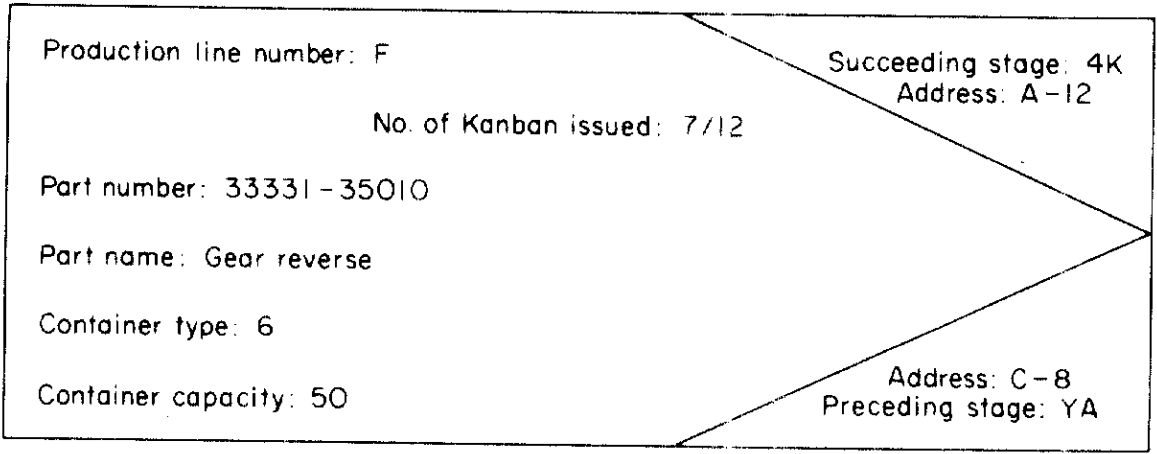
\includegraphics[width=11cm,angle=1,origin=c]{figure1.png}
\caption{看板设计}
\label{fig:layout}
\end{figure}
\end{enumerate}

\subsection{操作过程}

\subsubsection{过程内看板}

某阶段的零部件被放在一个容器里。一个看板被贴在或挂在容器上,然后把容器放在看板指定的储存地点(见图\ref{fig:in-process} \textcircled{1})。

当下游工序提取零部件或原材料时,工人把看板取下来,放在看板盒里(见图\ref{fig:in-process} \textcircled{2})。盒子里的看板被定期取出来挂在计划板的钩子上。计划板上各种看板的顺序向工人们展示了生产过程中各项任务的订单派送情况(见图\ref{fig:in-process} \textcircled{3})。

工人按照预先设计的速率,根据计划板上各种看板的顺序生产各种物品。看板自身也会随着某批产品投入生产而移动到生产过程中(见图\ref{fig:in-process} \textcircled{4})。

步骤\textcircled{1}到\textcircled{4}反复运行,生产过程也就持续有效地进行。

我们应该牢记,在步骤\textcircled{2}中,如果下游工序始终不提货,那么看板就不会进入看板盒或者挂上计划板。因此,这个车间就始终不会生产这种物品。

\begin{figure}[htbp]
\centering
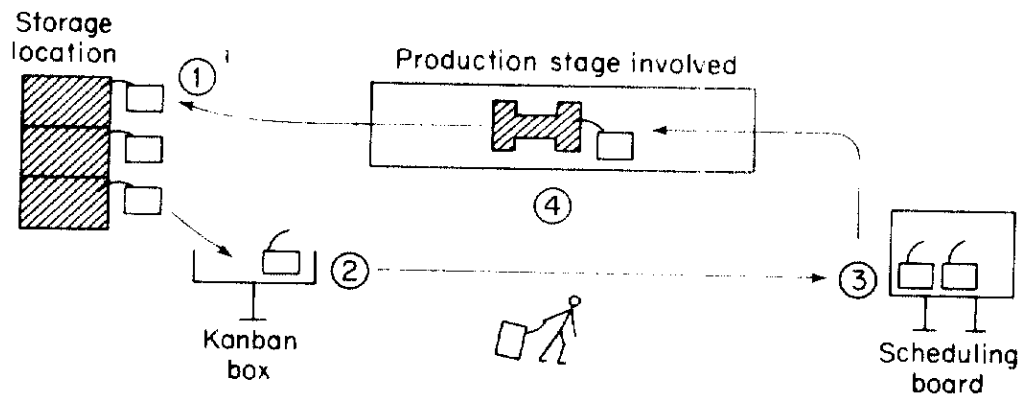
\includegraphics[width=13cm,angle=1,origin=c]{figure2.png}
\caption{过程内看板的循环}
\label{fig:in-process}
\end{figure}

\subsubsection{过程间看板}

过程间看板操作跟过程内看板是一样的,只要把运输视为类似于制造的操作就行了(图\ref{fig:inter-process})。

\begin{figure}[htbp]
\centering
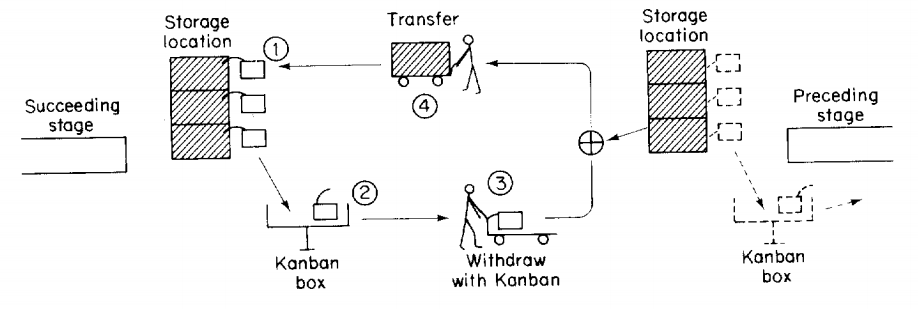
\includegraphics[width=14cm,angle=-1,origin=c]{figure3.png}
\caption{过程间看板的循环}
\label{fig:inter-process}
\end{figure}

我们同样应该牢记,提货数量等于看板表示的数量,盒子里没有看板就不会提取任何东西。

图3中的虚线表示过程内看板,它在上游车间中流动。当原材料或零部件从储存点被提走,容器上的过程内看板被替换为过程间看板。换下来的过程内看板会被放到过程内看板盒中。

正如我们在上面阐述的那样,下游生产过程的生产速率(数量)通过过程内看板和过程间看板传递给了上游工序。这样一个多阶段生产过程中的所有看板维持着所有阶段完成生产。





\section{系统模型}

我们按照如下说明,对拉式系统建模,以阐明系统特点。这里把系统考虑为只有一种产品的简单线性多阶段生产系统。

\subsection{标记方式}

\begin{tabbing}
空列 \= 标记 \= 意义 \kill
\>\> $t$ \' 时段。 \\
\>\> $O_t^n$ \' 第$n$道工序在$t$时段的订货量。 \\
\>\> $P_t^n$ \' 第$n$道工序在$t$时段的产量。 \\
\>\> $I_t^n$ \' 第$n$道工序在$t$时段末的库存。 \\
\>\> $M^n$ \' 订货单位(一个看板订多少)。 \\
\>\> $Z_t^n$ \' $I$除以$M$的余数。 \\
\>\> $C^n$ \' 第$n$道工序的生产能力。 \\
\>\> $L_1^n$ \' 看板从容器中拿出来的时间到开始生产的时间差。 \\
\>\> $L_2^n$ \' 生产开始和结束的时间差。 \\
\>\> $D_t$ \' $t$时段的需求。 \\
\>\> $D_{t,t+L}$ \' 在$t$时段末对$(t+L)$时段的需求预测。
\end{tabbing}

\subsection{信息和原材料流动示意图}

拉式系统中信息和原材料的流动可以用图\ref{fig:flow}来表示。

\begin{figure}[htbp]
\centering
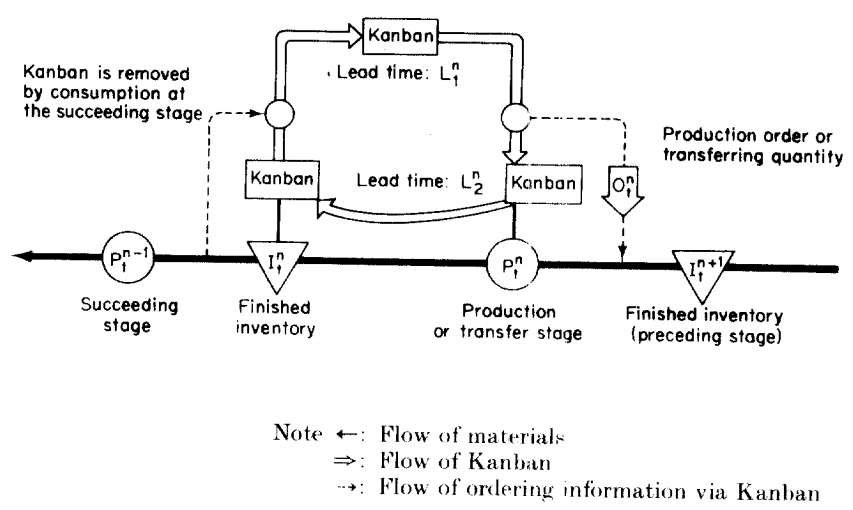
\includegraphics[width=13cm,angle=1,origin=c]{figure4.png}
\caption{拉式系统流程图}
\label{fig:flow}
\end{figure}

\subsection{系统的基本公式}

在拉式系统中,当容器里的物品开始被使用时,看板就从容器上取下来。因此,在每一个库存站都有这样一个容器,它里面的物品已经被使用了一部分,看板已经被取下来了。其他的容器里物品都是满的,看板也贴在上面。令$Z_t^n$为已经部分使用的容器中剩余物品数,记作
\[
Z_t^n=Mod(I_t^n, M^n)
\]
其中符号$Mod(A,B)$表示$A/B$的余数。第$n$个库存点已经移走的看板数由下游阶段的产量$P_t^{n-1}$决定。但是$P_t^{n-1}$的一部分可以被看板已移走的容器里的原材料抵消掉,这部分最多对应$Z_{t-1}^n$。

因此,可以用
\begin{equation}
\left.
\begin{aligned}
X &= P_t^{n-1}-Z_{t-1}^n & (P_t^{n-1} &\geqslant Z_{t-1}^n) \\
&\text{or} & \\
X &= 0 & (P_t^{n-1} &< Z_{t-1}^n)
\end{aligned}
\right\}
\label{eq:1}
\end{equation}
表示这个时段内移走的看板数所对应的原材料数。然后可以把第$t$时段移走的看板数表示为
\[
\left[\frac{X}{M^n}\right]_+ = \left[\frac{\max(0,P_t^{n-1}-Z_{t-1}^n)}{M^n}\right]_+
\]
符号$[A]_+$表示把$A$向上取整的高斯函数。经过$L_1^n$时间之后,被移走的看板会被添加到第$n$生产阶段的订单里。所以生产订单$O_t^n$为
\begin{equation}
O_t^n = \left[\frac{\max(0,P_{t-L_1^n}^{n-1}-Z_{t-L_1^n-1}^n)}{M^n}\right]_+M^n + O_{t-1}^n - P_{t-1}^n
\label{eq:2}
\end{equation}
其中$O_{t-1}^n - P_{t-1}^n$是前一时段末留下的未满足订单。生产量为
\begin{equation}
P_t^n = \min(O_t^n,C^n,I_{t-1}^{n+1}+P_{t-L_2^{n+1}}^{n=1})
\label{eq:3}
\end{equation}
其中$I_{t-1}^{n+1}+P_{t-L_2^n}^{n+1}$表示上游阶段的库存限制。

第$n$阶段的库存水平可以表示为
\begin{equation}
I_t^n=I_{t-1}^n+P_{t-L_2^n}^n-P_t^{n-1} \footnote{译者注:此处原文为$I_t^n=I_t^{n-1}+P_{t-L_2^n}^n-P_t^{n-1}$,疑为原作者笔误。}
\label{eq:4}
\end{equation}

以上公式(\ref{eq:2})-(\ref{eq:4})是拉式系统的基本公式。



\section{生产和库存的波动分析}

\subsection{单位订货量相对较小的情况}

\subsubsection{生产波动}

当单位订货量$M^n$与产量$P_t^n$相比相对较小时,我们可以令
\[
\left[\frac{\max(0,P_{t-L_1^n}^{n-1}-Z_{t-L_1^n-1}^n)}{M^n}\right]_+M^n \fallingdotseq P_{t-L_1^n}^{n-1}
\]
然后根据(\ref{eq:2})有
\begin{equation}
O_t^n \fallingdotseq P_{t-L_t^n}^{n-1} + O_{t-1}^n - P_{t-1}^n
\label{eq:5}
\end{equation}

当生产能力$C^n$和上游阶段库存$I_t^{n+1}$没有约束时,(\ref{eq:3})可以写作
\begin{equation}
P_t^n = O_t^n
\label{eq:6}
\end{equation}
由(\ref{eq:5})和(\ref{eq:6})可得
\begin{align}
P_t^n &= P_{t-L_1^n}^{n-1}\label{eq:7}\\
&=P_{t-(L_1^n+L_1^{n-1})}^{n-2}\notag\\
&\vdots\notag\\
&=P_{t-(L_1^n+L_1^{n-1}+\ldots+L_1^2)}^1\label{eq:8}
\end{align}

正如拉式系统中得出的这个结果,当单位订货量与产量相比相对较小时,下游阶段的生产波动始终按照原始情况传递给上游阶段。传递过程中的时滞等于流程中各阶段从容器上移走看板和开始生产之间的时差之和。

特别地,如果最终阶段$\{P^1\}$的生产是独立的,则$\{P_1^n\}$的方差为
\begin{equation}
V(P^n) = V(P^{n-1}) = \cdots = V(P^1)
\label{eq:9}
\end{equation}

定义放大率:
\[
\amp(p^n) = \frac{V(P^n)}{V(P_1)}
\]
根据(\ref{eq:9})
\begin{equation}
\amp(P^n) = \amp(P^{n+1}) = \cdots = 1
\label{eq:10}
\end{equation}

\subsubsection{库存波动}

根据(\ref{eq:7})
\[
P_{t-L_2^n}^n = P_{t-(L_1^n+L_2^n)}^{n-1}
\]
因此根据(\ref{eq:4})
\[
I_t^n = I_{t-1}^n + P_{t-(L_1^n+L_2^n)-P_t^{n-1}}-P_t^{n-1}\footnote{译者注:此处原文为$I_t^n = I_{t-1}^n + P_{t-(_1^n+L_2^n)-P_t^{n-1}}-P_t^{n-1}$,应为原作者笔误。}
\]
解这个方程可得
\begin{equation}
I_t^n = A - \sum_{R=t-(L_1^n+L_2^n)+1}^tP_R^{n-1}
\label{eq:11}
\end{equation}
其中
\[
A = I_0^n + \sum^{R \geqslant 0}P_R^{n-1}
\]
表示初始状态。

当$\{P_t^1\}$相互独立时,由(\ref{eq:1})可得
\begin{equation}
V(I^n) = (L_1^n+L_2^n)V(P^{n-1})
\label{eq:12}
\end{equation}

将(\ref{eq:9})代入(\ref{eq:12})可得
\begin{equation}
V(I^n) = (L_1^n + L_2^n)V(P^1)
\label{eq:13}
\end{equation}

令
\[
\amp(I^n) = \frac{V(I^n)}{V(P^1)}
\]
然后由(\ref{eq:13})可得
\begin{align}
\amp(I^n) &= \frac{V(I^n)}{V(P^1)} \notag \\
\amp(I^n) &= L_1^n + L_2^n \label{eq:14}
\end{align}
$L_1^n+L_2^n$表示从容器上移走看板直到该阶段完成生产的时间差。

因此,在拉式系统中,当$\{P_1\}$的波动独立时,每阶段的库存波动相比于最终阶段$\{P_1\}$来说是放大了。放大的程度随着看板从容器上取走的时间和该阶段完成生产的时间之差增大而增大。但是,放大的程度不会随某阶段在流水线上的位置越靠上而越大。

到目前为止,我们假设的是没有生产能力和库存水平的约束。如果这些约束存在,$\{P_t^n\}$的上限会受到$C^n$或者$I_t^{n+1}+P_{t-L_2^{n+1}}^{n+1}$的限制(见公式\ref{eq:3}),因此在这些情况下波动会比无约束情况下更小。但是,伴随着波动变小,未满足订单数和生产延迟都会变大。无论如何,这些管理问题不属于我们要研究的目标。

\subsection{单位订货量相对较大的情况}

在第$n$阶段单位订货量$M^n$与产量$P_{t-1}^n$相比较大的情况下,公式(\ref{eq:2})中的订货量\footnote{译者注:此处原文为“production quantity”,疑应为“order quantity”。}$O_t^n$不能按照公式(\ref{eq:5})那样近似,所以很难作出理论分析。因此,我们尝试用以下仿真模型进行分析。

\subsubsection{标记方式}

\begin{tabbing}
空列 \= 标记 \= 意义 \kill
\>\> $O_t^n$ \' 在$t$时段,第$(n-1)$阶段向第$n$阶段订货的数量。 \\
\>\> $R_t^n$ \' 在$t$时段,第$n$阶段向第$(n-1)$阶段运货的数量。 \\
\>\> $B_t^n$ \' $t$时段末,从第$(n+1)$阶段的库存运到第$n$阶段,正等待处理的数量。 \\
\>\> $L_{P_1}^n$ \' 与前面定义的$L_1^n$意义相同。 \\
\>\> $L_{P_2}^n$ \' 与前面定义的$L_2^n$意义相同。 \\
\>\> $L_{H_1}^n$ \' 从容器上取走看板直到订单开始发货的时长。 \\
\>\> $L_{H_2}^n$ \' 从订单开始发货到操作完成的时长。 \\
\>\> $S^0$ \' 最终阶段的安全库存。
\end{tabbing}

除了以上定义的标记,其余标记与之前定义的相同。

\subsubsection{仿真模型}

\begin{enumerate}

\item
一般模型;如图\ref{fig:model}所示。

这是包含$n$个生产阶段和$n$个运输阶段的单产品多阶段生产过程。

\item
最终产品的需求量$D_t$;服从均值为$\bar{D}$,方差为$\sigma_D^2$的正态分布。均值和方差都是已知的。

\item
生产和运输计时;生产和运输在每个时段初开始。

\item
系统中的公式

最终阶段的库存量
\begin{equation}
B_t^0 = B_{t-1}^0 + R_{t-L_{H_2}^1}^1 - D_1
\label{eq:15}
\end{equation}

产品的运送
\begin{equation}
R_t^1 = I_{t-1}^1
\label{eq:16}
\end{equation}

运送前的库存
\begin{equation}
I_t^1 = P_{t-L_{P_2}^1}^1
\label{eq:17}
\end{equation}

第一阶段的订货量。

(我们只对最终阶段采用推式系统。)
\begin{equation}
O_t^1 = \hat{D}_{t-1,t+L} + \hat{D}_{t-1,t+L-1} - P_{t-1}^1 - B_{t-1}^0 + S^0
\label{eq:18}
\end{equation}
其中$L=L_{P_2}^1+L_{H_2}^1$。

第二阶段的生产、运输、库存公式可以用上面提到的方法得到。

\end{enumerate}

\begin{landscape}
\begin{figure}[p]
\centering
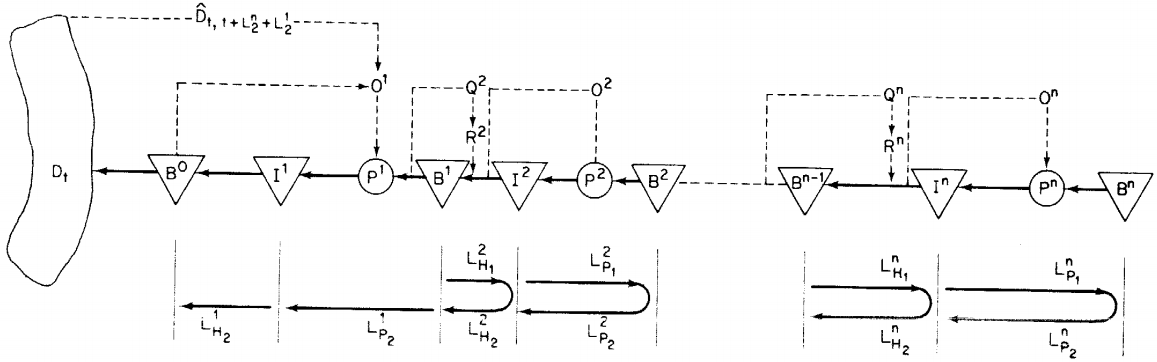
\includegraphics[width=21cm,angle=1,origin=c]{figure5.png}
\caption{仿真模型概念图}
\label{fig:model}
\end{figure}
\end{landscape}

\subsubsection{输入数据和参数值}

\begin{tabbing}
编号 \= 变量啊变量 \= 值\kill
(1) \> $t$ \> $1,2,3,\ldots,100$ \\
(2) \> $D_t$ \> $\bar{D}=100\frac{\sigma_D}{\bar{D}}=0.1$ \\
(3) \> $\hat{D}$ \> $\bar{D}$ \\
(4) \> $n$ \> 5 \\
(5) \> $I_0^n,C^n$ \> very large numbers \\
(6) \> $L_{P_1}^n=L_{P_2}^n=L_{H_1}^n=L_{H_2}^n=0$ ($n=1,2,\ldots,5$)
\end{tabbing}

\subsubsection{实验结果}

在上述条件下,改变单位订货量$M^n$,结果如图\ref{fig:influence-M-P}和图\ref{fig:influence-M-I}所示。

\begin{figure}[htbp]
\centering
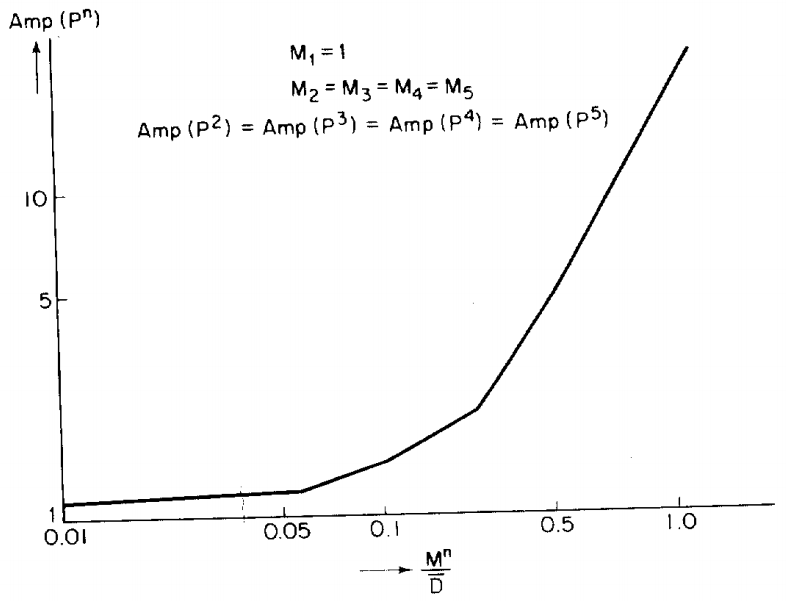
\includegraphics[width=11cm,angle=-1.5,origin=c]{figure6.png}
\caption{单位订货量$M^n$对生产波动的影响}
\label{fig:influence-M-P}
\end{figure}

\begin{figure}[htbp]
\centering
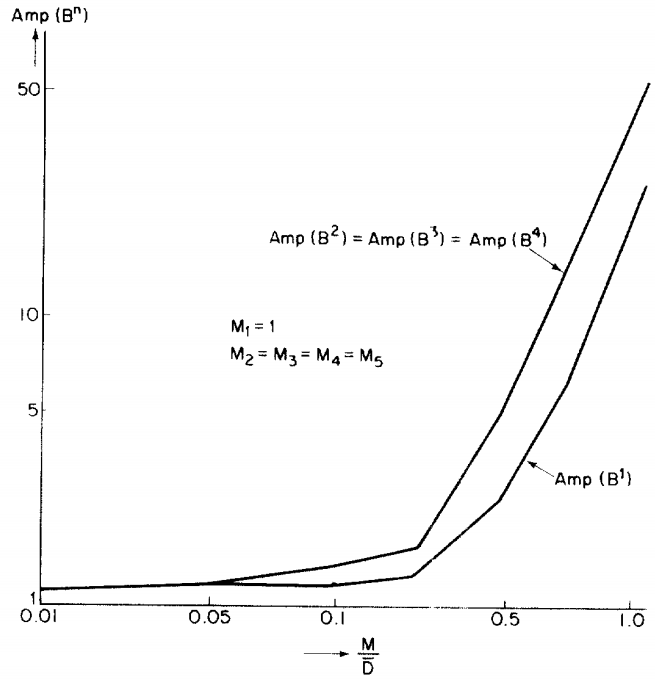
\includegraphics[width=10cm,angle=1,origin=c]{figure7.png}
\caption{单位订货量$M^n$对库存波动的影响}
\label{fig:influence-M-I}
\end{figure}

在拉式系统中,随着单位订货量相对于产量水平增大,生产和库存的波动会增大,但是波动不会在向上游传递的过程中扩大。

\subsection{与推式系统的比较}

为了比较推式系统和拉式系统内下游阶段生产波动对上游阶段的影响,推式系统(由早稻田大学的Y.Tanaka和T.Tabe建立)和本研究中的拉式系统的实验结果用图\ref{fig:amp-P}和图\ref{fig:amp-I}展示。

\begin{figure}[htbp]
\centering
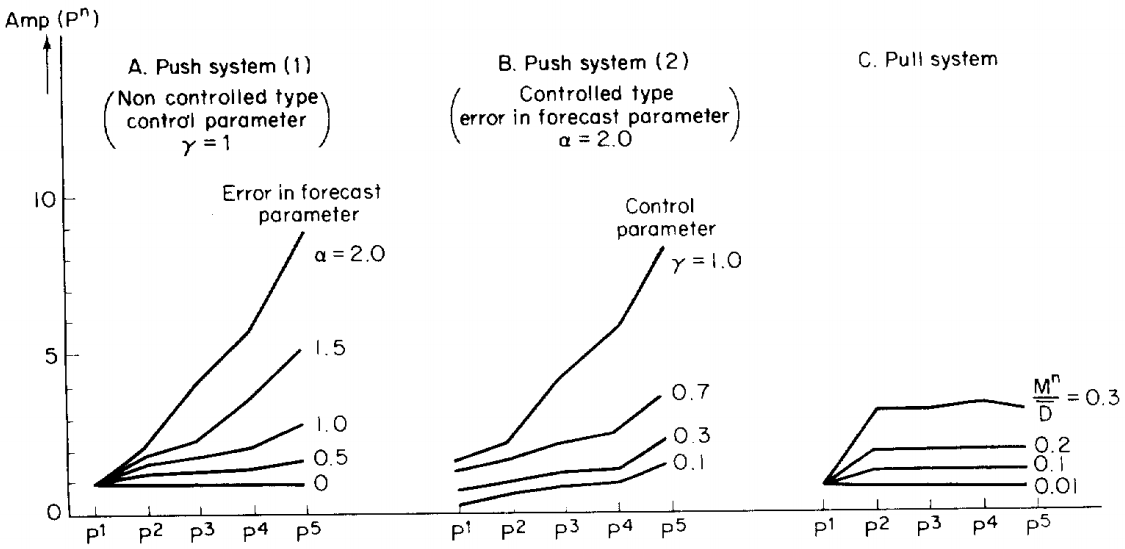
\includegraphics[width=14cm,angle=-0.5,origin=c]{figure8.png}
\caption{生产波动放大率}
\label{fig:amp-P}
\end{figure}

\begin{figure}[htbp]
\centering
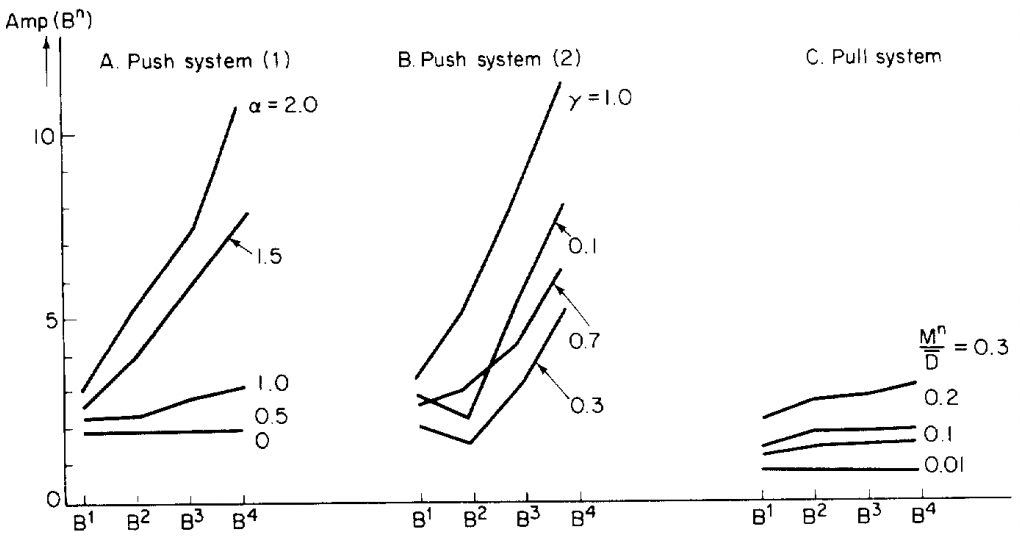
\includegraphics[width=14cm,angle=-0.5,origin=c]{figure9.png}
\caption{库存波动放大率}
\label{fig:amp-I}
\end{figure}

输入数据和参数是相同的,除了$L_{P_1}^n=0$, $L_{P_2}^n=1$, $L_{H_1}^n=1$, $L_{H_2}^n=0$,以及推式系统中的单位订货量$M$始终为1。推式系统模型的细节展示在Muramatsu及其他人的文献中。

正如这些图表所示,在推式系统中,波动在上游变得更大。这是预测误差的结果。因此,有必要在推式系统中让控制参数保持在正确的水平。另一方面,在拉式系统中,波动放大率随着单位订货量的增大而增大。因此,试图让单位订货量最小化是有必要的。




\section{总结}

\begin{enumerate}
\item
在拉式系统中,单位订货量的大小非常重要。在单位订货量与产量水平相比很小的情况下,生产波动不会在上游阶段放大。单位订货量较大时会造成波动的放大,但即使是这种情况下,放大率也不会继续向上游阶段扩大。

\item
在推式系统中,生产和库存波动的放大率取决于预测误差的影响。当考虑放大率时,推式系统和拉式系统之间的抉择取决于预测误差的程度。

\item
拉式系统中另一个影响放大率的参数是从容器上移走看板到阶段生产完成的“提前期”。提前期越长,放大率越高。
\end{enumerate}


\nocite{ref1}
\nocite{ref2}
\nocite{ref3}



致谢:我们希望向早稻田大学的Rintaro Muramatsu博士致以诚挚的感谢,他提出了重要的指导和建议。

\begin{thebibliography}{99}

\bibitem{ref1} Kusunoki, K.,and Sugimori, Y., Fourth International Conference on Production Research, Five Paper Sessions.

\bibitem{ref2} Magee, J.F., Production planning and inventory control.

\bibitem{ref3} Muramatsu, R., Tannaka, Y., and Tabe, T., Analysis of production order and inventory fluctuations, Fifth International Conference on Production Research, Free Paper Sessions.



\end{thebibliography}
















\chapter{汽车销售数据}

% Table generated by Excel2LaTeX from sheet 'Sheet1'
\begin{table}[htbp]
  \centering
  \caption{汽车销售数据}
    \begin{tabular}{ccccc}
    \toprule
    \textbf{time} & LIVINA & TIIDA & EXCELLE & EXCELLEXT \\
    \midrule
    \textbf{2012/1/1} & \textbf{9021} & \textbf{13295} & \textbf{15189} & \textbf{4598} \\
    \textbf{2012/2/1} & \textbf{8423} & \textbf{15311} & \textbf{9247} & \textbf{2643} \\
    \textbf{2012/3/1} & \textbf{7728} & \textbf{15627} & \textbf{10049} & \textbf{4015} \\
    \textbf{2012/4/1} & \textbf{8166} & \textbf{14128} & \textbf{8306} & \textbf{3675} \\
    \textbf{2012/5/1} & \textbf{10315} & \textbf{16334} & \textbf{8750} & \textbf{3235} \\
    \textbf{2012/6/1} & \textbf{14298} & \textbf{18691} & \textbf{11000} & \textbf{4228} \\
    \textbf{2012/7/1} & \textbf{6484} & \textbf{15167} & \textbf{9807} & \textbf{3305} \\
    \textbf{2012/8/1} & \textbf{8527} & \textbf{11047} & \textbf{11024} & \textbf{4012} \\
    \textbf{2012/9/1} & \textbf{3773} & \textbf{8246} & \textbf{11306} & \textbf{4005} \\
    \textbf{2012/10/1} & \textbf{1866} & \textbf{5173} & \textbf{12000} & \textbf{4541} \\
    \textbf{2012/11/1} & \textbf{3780} & \textbf{5649} & \textbf{13209} & \textbf{4507} \\
    \textbf{2012/12/1} & \textbf{5343} & \textbf{5544} & \textbf{7688} & \textbf{2973} \\
    \textbf{2013/1/1} & \textbf{3731} & \textbf{10458} & \textbf{17873} & \textbf{5821} \\
    \textbf{2013/2/1} & \textbf{128} & \textbf{6838} & \textbf{11135} & \textbf{3159} \\
    \textbf{2013/3/1} & \textbf{25} & \textbf{8192} & \textbf{13287} & \textbf{3366} \\
    \textbf{2013/4/1} & \textbf{6607} & \textbf{8062} & \textbf{14279} & \textbf{4134} \\
    \textbf{2013/5/1} & \textbf{6684} & \textbf{9938} & \textbf{12202} & \textbf{4208} \\
    \textbf{2013/6/1} & \textbf{5508} & \textbf{12711} & \textbf{10128} & \textbf{4404} \\
    \textbf{2013/7/1} & \textbf{6417} & \textbf{10930} & \textbf{12001} & \textbf{5183} \\
    \textbf{2013/8/1} & \textbf{5604} & \textbf{7781} & \textbf{13023} & \textbf{5075} \\
    \textbf{2013/9/1} & \textbf{9965} & \textbf{15555} & \textbf{13790} & \textbf{5855} \\
    \textbf{2013/10/1} & \textbf{33} & \textbf{13281} & \textbf{11903} & \textbf{5084} \\
    \textbf{2013/11/1} & \textbf{12597} & \textbf{12818} & \textbf{14612} & \textbf{5265} \\
    \textbf{2013/12/1} & \textbf{5318} & \textbf{12761} & \textbf{6288} & \textbf{2199} \\
    \textbf{2014/1/1} & \textbf{6327} & \textbf{8818} & \textbf{26834} & \textbf{7342} \\
    \textbf{2014/2/1} & \textbf{5090} & \textbf{8151} & \textbf{13223} & \textbf{3037} \\
    \textbf{2014/3/1} & \textbf{4585} & \textbf{7640} & \textbf{17687} & \textbf{5328} \\
    \textbf{2014/4/1} & \textbf{6253} & \textbf{10832} & \textbf{13744} & \textbf{4509} \\
    \bottomrule
    \end{tabular}%
  \label{tab:汽车销售数据}%
\end{table}%




















